\documentclass{article}

\usepackage{enumitem}
\usepackage{graphicx}
\usepackage{verbatim}
\usepackage{booktabs}
\usepackage{algorithm}
\usepackage{algpseudocode}
%\algnewcommand\Return{\State \textbf{return} } % Adds native \Return support

\usepackage[colorlinks=true]{hyperref}
% \hypersetup{
    %     colorlinks=true,
    %     linkcolor=blue,
    %     citecolor=blue,
    %     filecolor=blue,
    %     urlcolor=blue
    % }

\usepackage[table,dvipsnames]{xcolor}
\usepackage{authblk}
\usepackage[a4paper, margin=1in]{geometry}
\usepackage{amsmath}
\usepackage{amsthm}
\usepackage{wrapfig}
\usepackage{subcaption}
\usepackage{multirow}
\usepackage{listings}
\definecolor{customblue}{RGB}{0, 76, 153}
\definecolor{softgreen}{RGB}{226, 245, 236}
\definecolor{softred}{RGB}{255, 232, 232}
\definecolor{softyellow}{RGB}{255, 247, 214}
\DeclareMathOperator*{\argmax}{arg\,max}

% \lstset{
%     basicstyle=\ttfamily\small,
%     keywordstyle=\color{customblue}\bfseries,
%     commentstyle=\color{teal!70!black},
%     stringstyle=\color{red!70!black},
%     frame=single,
%     breaklines=true,
%     showstringspaces=false,
%     columns=fullflexible
% }
\lstset{
    language=Python,
    backgroundcolor=\color{gray!10},   % Light gray background
    basicstyle=\ttfamily\small,        % Monospace font
    keywordstyle=\color{blue}\bfseries,% Blue bold keywords
    commentstyle=\color{green!60!black},% Dark green comments
    showspaces=false,                  % Don't show spaces
    showstringspaces=false,            % Don't show spaces in strings
    frame=single,                      % Add a frame around the code
    numbers=left,                      % Line numbers on the left
    numberstyle=\tiny\color{gray}      % Line number style
}
\usepackage[backend=biber, style=numeric]{biblatex}
\addbibresource{dna_storage_refs.bib}

\newcommand{\dt}[1]{\frac{\mathrm{d}#1}{\mathrm{d}t}}

\newcommand{\be}{\begin{equation}}
\newcommand{\ee}{\end{equation}}


\begin{document}
\title{\textcolor{blue!30!black}{\textsf{A Library in a Droplet}}\\
    \large How Digital Files Can Be Written into DNA }
\author[1]{George M. Church}
\author[2]{Nick Goldman}

\affil[1]{Harvard Medical School, Boston, USA }
\affil[2]{European Bioinformatics Institute, Hinxton, UK}

\maketitle


\section{Can a File Become a Molecule?}

What would a library look like if its pages were replaced by molecules? Instead of shelves and hard
drives, imagine a tiny tube containing millions of invisible DNA strands. The idea sounds like science
fiction, yet researchers have already stored books, images, audio, software, and other digital files in
synthetic DNA \cite{church2012}.

DNA normally carries biological instructions, but its four-letter alphabet can also carry arbitrary
computer data. The DNA need not be placed inside a living organism: it may be synthesized, dried,
stored, and later read by a sequencing machine. The central idea is simple:

\begin{quote}
    Convert bits into DNA letters, preserve the molecules, and reverse the conversion when the file is needed again.
\end{quote}

\begin{figure}[h]
    \centering
    % \hfill
    \begin{subfigure}[t]{0.32\textwidth}
        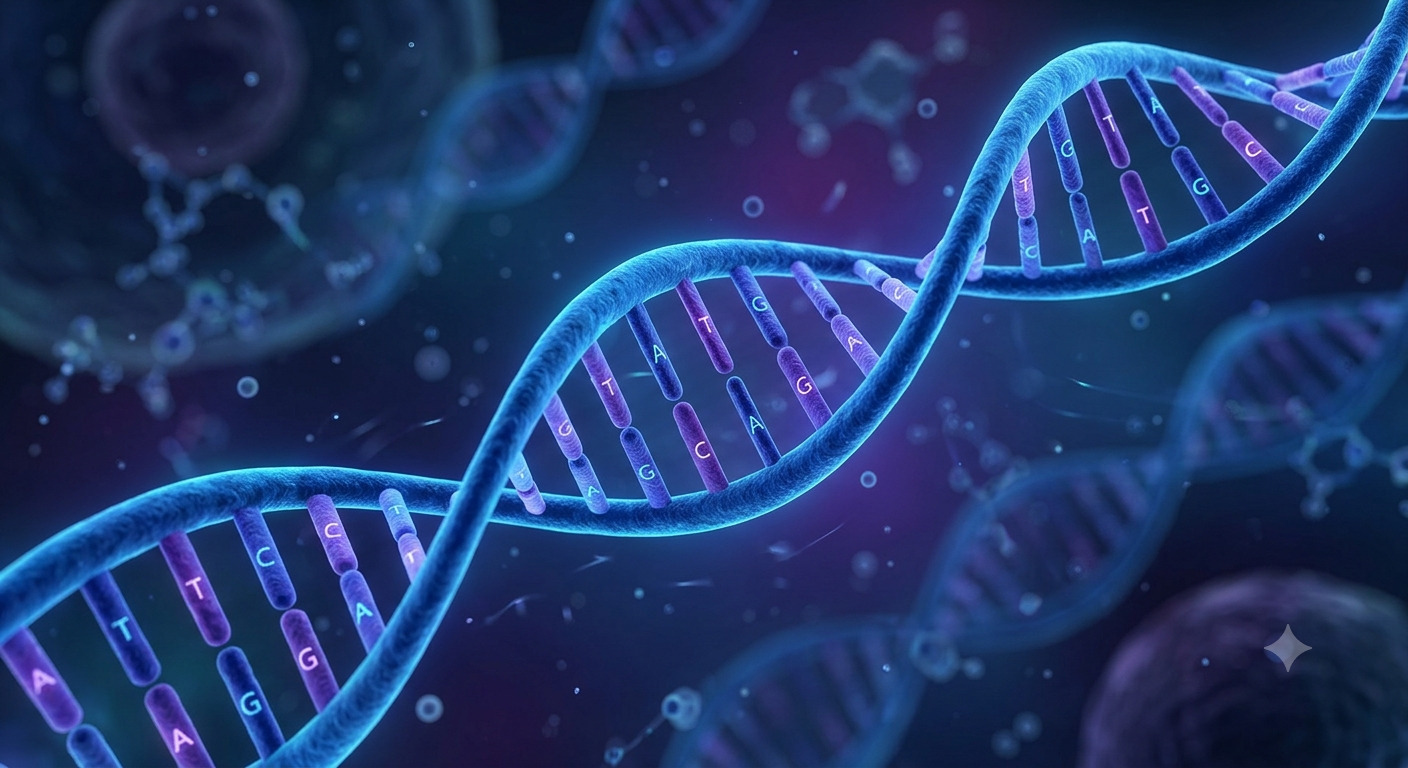
\includegraphics[width=\linewidth]{1-dna.jpg}
        \caption{DNA as a biological molecule.}
        \label{fig:1-dna}
    \end{subfigure}
    \hfill
    \begin{subfigure}[t]{0.32\textwidth}
        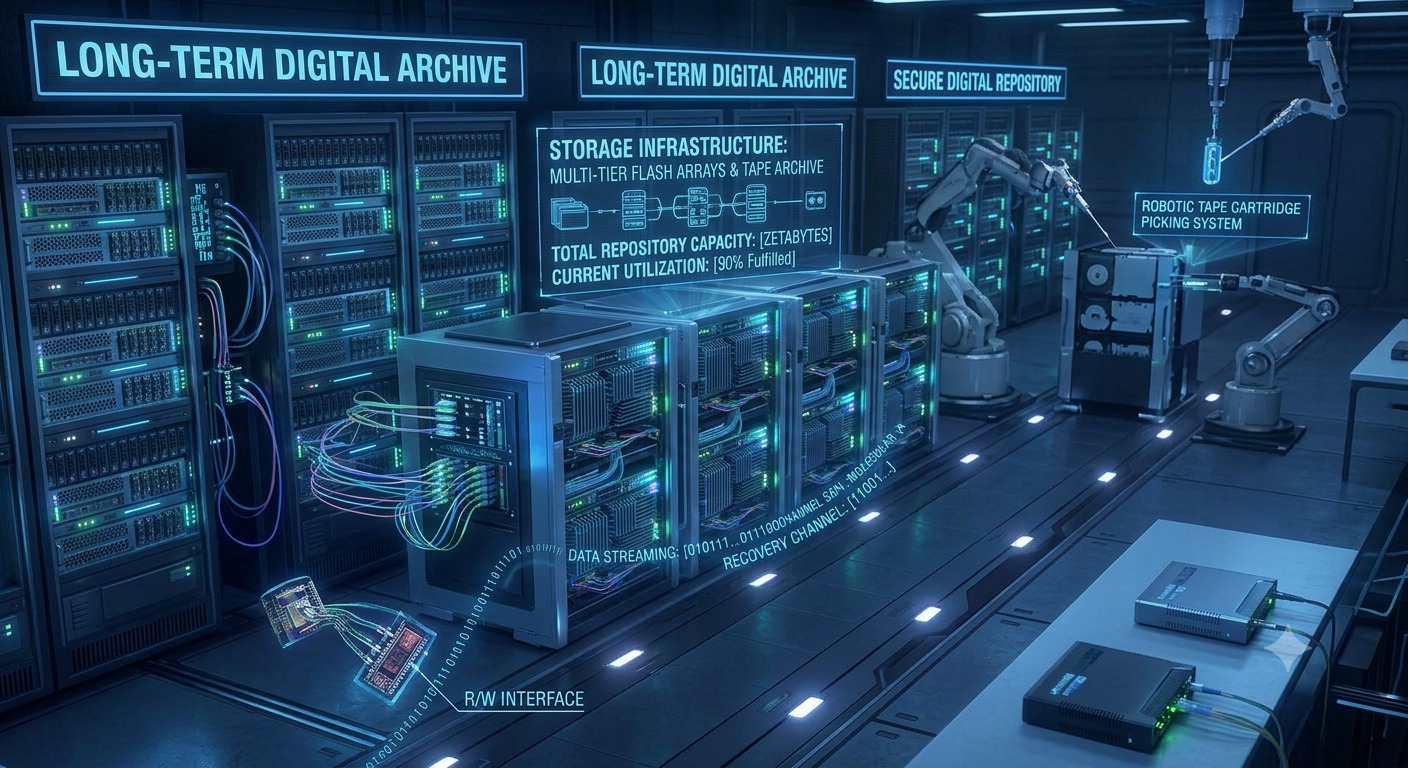
\includegraphics[width=\linewidth]{2-data.jpg}
        \caption{Digital data represented in bits.}
        \label{fig:2-data}
    \end{subfigure}
    \hfill
    \begin{subfigure}[t]{0.32\textwidth}
        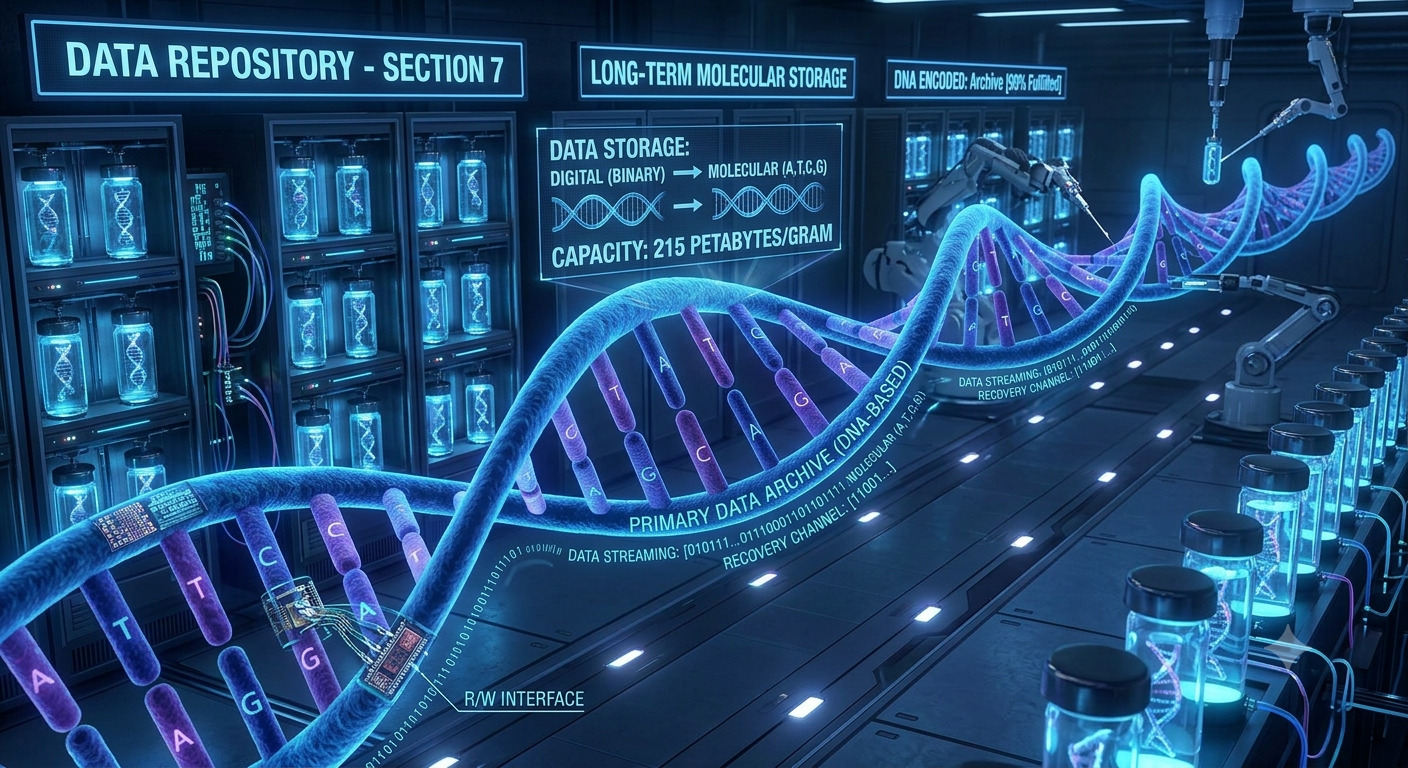
\includegraphics[width=\linewidth]{3-dna-as-data.jpg}
        \caption{DNA used as a storage medium.}
        \label{fig:3-dna}
    \end{subfigure}

    \vspace{0.5cm}

    % second row
    \begin{subfigure}{\textwidth}
        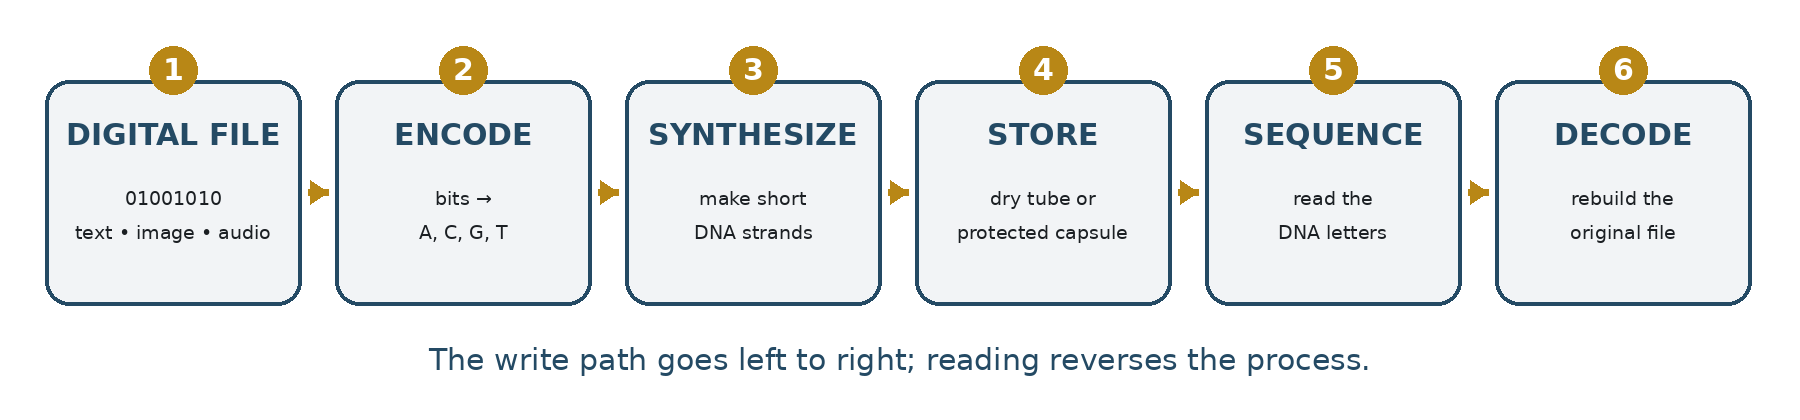
\includegraphics[width=\linewidth]{dna_storage_pipeline.png}
        \caption{A simplified DNA data-storage cycle, from a digital file to synthetic DNA and back again.}
        \label{fig:pipeline}
    \end{subfigure}

    \caption{From biological DNA to a complete DNA-based digital storage system.}
    \label{fig:system}
\end{figure}

The six stages in fig.~\ref{fig:pipeline} separate the electronic world from the molecular one. The computer performs
the encoding and decoding; laboratory instruments perform the writing and reading.

\subsection{A Four-Letter Storage Medium}
Ordinary digital files are sequences of bits, each equal to 0 or 1. DNA uses four symbols:
\[
    \mathcal{A} = \{ \text{A, C, G, T} \}
\]

Because four symbols can represent four binary pairs,
\be
4^n = (2^2)^n = 2^{2n}
\ee

\begin{table}
    \centering
    \caption{One possible conversion from binary pairs to DNA bases.}
    \begin{tabular}{cc}
        \toprule
        \rowcolor{gray!20} \textbf{Binary pair} & \textbf{DNA base} \\
        \midrule
        00                                      & A                 \\
        01                                      & C                 \\
        10                                      & G                 \\
        11                                      & T                 \\
        \bottomrule
    \end{tabular}
    \label{tab:one}
\end{table}

so an ideal DNA symbol can carry two bits of information.
Table 1 gives one possible toy mapping. Other mappings are equally valid.
For example, the character A has binary code \texttt{01000001} in ASCII.\footnote{ASCII is a standard numerical representation for common text characters.} Grouping the bits in pairs and using
Table \ref{tab:one} gives
\begin{equation}
    \texttt{A} \rightarrow \texttt{01 00 00 01} \rightarrow \texttt{CAAC}
\end{equation}

This example explains the principle, but a real DNA-storage system needs more structure than a direct
translation.


\section{Building a Molecular File}
Long files are divided into many short DNA strands called oligonucleotides, or oligos. Each oligo
contains not only data but also information that helps the system locate and reconstruct it.
% \begin{center}
%     \boxed{LEFT PRIMER} \quad \boxed{ADDRESS}  \quad \boxed{DATA PAYLOAD}  \quad \boxed{CHECK STATUS}  \quad \boxed{RIGHT PRIMER}
% \end{center}
\begin{center}
    \ttfamily\small
    \fbox{\strut LEFT PRIMER}\hspace{2mm}
    \fbox{\strut ADDRESS}\hspace{2mm}
    \fbox{\strut DATA PAYLOAD}\hspace{2mm}
    \fbox{\strut CHECK SYMBOLS}\hspace{2mm}
    \fbox{\strut RIGHT PRIMER}
\end{center}
If the corresponding lengths are $L_p, L_a, L_d$, and $L_c$, then the total strand length is
\begin{equation}
    L = 2L_p + L_a + L_d + L_c
    \label{eqn:three}
\end{equation}
The complete storage cycle can be summarized in five steps:

\begin{enumerate}[label=\Roman*.]
    \item \textbf{Encoding:} convert a file into carefully designed DNA sequences.
    \item \textbf{Synthesis:} manufacture those sequences as physical molecules.
    \item \textbf{Preservation:} keep the DNA dry, cold, or chemically protected \cite{erlich2017}.
    \item \textbf{Sequencing:} read many copies of the stored strands.
    \item \textbf{Reconstruction:} order the fragments, correct errors, and rebuild the original file.
\end{enumerate}

Primer regions can also support random access: instead of reading an entire DNA pool, a user can
request one particular file. In one large experiment, researchers stored more than 200 MB across 35
files and recovered each file individually \cite{grass2015}.

\section{Addresses, Payload, and Useful Capacity}
Suppose a file is divided among M DNA strands. To assign a distinct address to every strand, the
required address length is

\begin{equation}
    L_a = \lceil \log_4 M \rceil,
\end{equation}
because an address of $L_a$ DNA bases can represent $4^{L_a}$ different positions.

Using the strand structure in eq. \ref{eqn:three}, the number of bases available for actual file data is
\begin{equation}
    L_d = L - 2L_p - L_a - L_c
\end{equation}
Since one DNA base can ideally represent two bits, a file containing B bits requires approximately
\begin{equation}
    M = \left\lceil \frac{B}{2L_d}  \right\rceil
\end{equation}
DNA strands. Thus, longer addresses and stronger error protection improve reliability, but leave less
room for the data payload.
\section{A Compact Encoding Procedure}
The following procedure converts a bit string into addressed DNA strands. Here, Enc(·) applies the
mapping in Table\ref{tab:one}, and $\parallel$ denotes concatenation.

% \begin{algorithm}
%     \caption{Create addressed DNA strands}
%     \label{alg:one}
%     \begin{algorithmic}[1]
%         \Require Bit string $x$, payload size $q$, and primers $P_L, P_R$
%         \Procedure{Create addressed DNA strands}
%         \For{each $q$-bit block $x_i$ \textbf{do}}
%             \State $a_i \leftarrow$ base-4 adrress of $i$,   $d_i\leftarrow \text{Enc}(x)$
%             \State $c_i \leftarrow \text{Checksum}(a_i\parallel d_i)
%             \State $s_i \leftarrow P_L \parallel a_i \parallel d_i \parallel c_i \parallel P_R
%         \EndFor
%         \Return \(s_1, s_2, \ldots, s_M \)
%         \EndProcedure
%     \end{algorithmic}
% \end{algorithm}
\begin{algorithm}
    \caption{Create addressed DNA strands}
    \label{alg:one}
    \begin{algorithmic}[1]
        \Require Bit string $x$, payload size $q$, and primers $P_L, P_R$
        \Procedure{CreateAddressedStrands}{$x, q, P_L, P_R$}
        \For{each $q$-bit block $x_i$}
        \State $a_i \leftarrow$ base-4 address of $i$, $d_i\leftarrow \text{Enc}(x)$
        \State $c_i \leftarrow \text{Checksum}(a_i\parallel d_i)$
        \State $s_i \leftarrow P_L \parallel a_i \parallel d_i \parallel c_i \parallel P_R$
        \EndFor
        \State \textbf{return} \(s_1, s_2, \ldots, s_M \)
        \EndProcedure
    \end{algorithmic}
\end{algorithm}

\section{\textcolor{blue}{Why the Obvious Code Is Not Enough}}

The direct mapping in Table \ref{tab:one} is useful for learning, but biological hardware does not treat every DNA
string equally well


\subsection{Sequence Constraints}
Three common design concerns are:

\begin{enumerate}[label=$\diamond$]
    \item Long repetitions: strings such as \texttt{AAAAAAA} are difficult to synthesize and read accurately.
    \item Unbalanced composition: strands with extremely high or low proportions of G and C may behave poorly in laboratory procedures.
    \item Lost ordering: millions of strands are mixed together, so each fragment needs an address.
\end{enumerate}

For a DNA string s, its GC percentage is
\begin{equation}
    \text{GC}(s) = \frac{N_G(s) + N_C(s)}{|s|} \times 100\%
\end{equation}
where $NG(s)$ and $NC(s)$ count the two bases. Real encoders search for strings that carry the required
bits while avoiding problematic patterns.



\subsection{Errors at Different Stages}
A stored strand can be altered in several ways:

\begin{align*}
    \centering
    \textbf{Original }     & \texttt{ACGTAC}  \\
    \textbf{Substitution } & \texttt{ACCTAC}  \\
    \textbf{Insertion }    & \texttt{ACGTTAC} \\
    \textbf{Deletion }     & \texttt{ACTAC}   \\
\end{align*}

\begin{table}[h]
    \caption{Where DNA-storage errors arise and how systems respond.}
    \label{tab:two}
    \resizebox{\linewidth}{!}{%
        \begin{tabular}{cllll}
            \toprule
            \multirow{2}{*}{\textbf{Phase}}   & \multirow{2}{*}{\textbf{Stage}} & \multicolumn{3}{c}{\textbf{Challenge and response}}                                                           \\
            \cmidrule{3-5}
                                              &                                 & \textbf{Problem}                                    & \textbf{Effect}           & \textbf{Response}           \\
            \midrule
            \multirow{2}{*}{\textbf{Writing}} & \textbf{Encoding}               & Repeats or extreme GC content                       & Poor synthesis or reading & Choose another sequence     \\
                                              & \textbf{Synthesis}              & Base errors                                         & INcorrect stand           & Add checks and copoies      \\
            \midrule
            \textbf{Preservation}             & \textbf{Storage}                & Damage or strand loss                               & Missing fragments         & Protect DNA and keep copies \\
            \bottomrule
        \end{tabular}
    }
\end{table}


\section{Redundancy Without the Heavy Machinery}
Error-correcting codes can become mathematically sophisticated, but their basic purpose is easy to see:
store a little extra information so that imperfect reads do not destroy the message.

Suppose three sequencing reads report:
\begin{align*}
    \texttt{Read 1:} & \texttt{ACGTAC} \\
    \texttt{Read 2:} & \texttt{ACGTAC} \\
    \texttt{Read 3:} & \texttt{ACCTAC} \\
    % \caption{\textbf{Recovered sequence:} ACGTAC}
\end{align*}

A position-by-position majority vote repairs the single disagreement. Real systems combine this idea
with checksums, overlapping fragments, and stronger codes. The DNA Fountain system, for example,
stored about 2.14 MB of digital data and recovered it perfectly using a robust coding architecture \cite{organick2018}.

\textcolor{red}{The extra DNA is not wasted space; it is insurance against missing and corrupted molecules.}



\printbibliography

\end{document}
